%%**************************************************************
%% Vorlage fuer Bachelorarbeiten (o.ä.) der DHBW
%%
%% Autor: Tobias Dreher, Yves Fischer
%% Datum: 06.07.2011
%%
%% Autor: Michael Gruben
%% Datum: 15.05.2013
%%**************************************************************
\documentclass[%
	enabledeprecatedfontcommands,
	pdftex,
	oneside,		% Einseitiger Druck.
	12pt,			% Schriftgroesse
	parskip=half,	% Halbe Zeile Abstand zwischen Absätzen.
	headsepline,	% Linie nach Kopfzeile.
	footsepline,	% Linie vor Fusszeile.
	abstracton,	    % Abstract Überschriften
	ngerman,		% Translator
]{scrreprt}
%!TEX root = ../dokumentation.tex

%
% Nahezu alle Einstellungen koennen hier getaetigt werden
%



%Seitengroesse
\usepackage{fullpage}

%Zeilenumbruch und mehr
\usepackage[activate]{microtype}

% Zeichencodierung
\usepackage[utf8]{inputenc}
\usepackage[T1]{fontenc}

% Zeilenabstand
\usepackage[onehalfspacing]{setspace}

% Index-Erstellung
\usepackage{makeidx}

% Lokalisierung (neue deutsche Rechtschreibung)
\usepackage[ngerman]{babel}

% Anführungszeichen 
\usepackage[babel,german=quotes]{csquotes}
%\usepackage[style=swiss]{csquotes}


% Spezielle Tabellenform fuer Deckblatt
\usepackage{longtable}
\setlength{\tabcolsep}{10pt} %Abstand zwischen Spalten
\renewcommand{\arraystretch}{1.5} %Zeilenabstand

% Grafiken
\usepackage{graphicx}

\usepackage{tabularx}
\usepackage{multirow}

% Mathematische Textsaetze
%\usepackage{amsmath}
%\usepackage{amssymb}

% Pakete um Textteile drehen zu können, oder eine Seite Querformat anzeigen kann.
%\usepackage{rotating}
%\usepackage{lscape}

% Farben
\usepackage{color}
\definecolor{LinkColor}{rgb}{0,0,0.2}
\definecolor{ListingBackground}{rgb}{0.92,0.92,0.92}

\newcommand{\pdftitel}{Internet of Things}
\newcommand{\autor}{Dana Frey  \space Jonas Graubner \space  Maximilian Trumpp \space   Robin Ziegler}
\newcommand{\arbeit}{Laborarbeit}

% Titel, Autor und Datum
\title{\titel}
\author{\autor}
\date{\datum}

% PDF Einstellungen
\usepackage[%
	pdftitle={\pdftitel},
	pdfauthor={\autor},
	pdfsubject={\arbeit},
	pdfcreator={pdflatex, LaTeX with KOMA-Script},
	pdfpagemode=UseOutlines, % Beim Oeffnen Inhaltsverzeichnis anzeigen
	pdfdisplaydoctitle=true, % Dokumenttitel statt Dateiname anzeigen.
	pdflang=de % Sprache des Dokuments.
]{hyperref} 

% (Farb-)einstellungen für die Links im PDF
\hypersetup{%
	colorlinks=true, % Aktivieren von farbigen Links im Dokument
	linkcolor=LinkColor, % Farbe festlegen
	citecolor=LinkColor,
	filecolor=LinkColor,
	menucolor=LinkColor,
	urlcolor=LinkColor,
	bookmarksnumbered=true % Überschriftsnummerierung im PDF Inhalt anzeigen.
}

% Literaturverweise nach Harvard (mit deutschem und)
\usepackage[dcucite]{harvard}
\renewcommand{\harvardand}{und}

% Verschiedene Schriftarten
%\usepackage{goudysans}
%\usepackage{lmodern}
%\usepackage{libertine}
\usepackage{palatino} 

% Hurenkinder und Schusterjungen verhindern
% http://projekte.dante.de/DanteFAQ/Silbentrennung
\clubpenalty=10000
\widowpenalty=10000
\displaywidowpenalty=10000

% Quellcode
\usepackage{listings}
\lstloadlanguages{Java}
\lstset{%
	language=PHP,		 	 % Sprache des Quellcodes
	%numbers=left,           % Zelennummern links
	stepnumber=1,            % Jede Zeile nummerieren.
	numbersep=5pt,           % 5pt Abstand zum Quellcode
	numberstyle=\tiny,       % Zeichengrösse 'tiny' für die Nummern.
	breaklines=true,         % Zeilen umbrechen wenn notwendig.
	breakautoindent=true,    % Nach dem Zeilenumbruch Zeile einrücken.
	postbreak=\space,        % Bei Leerzeichen umbrechen.
	tabsize=2,               % Tabulatorgrösse 2
	basicstyle=\ttfamily\footnotesize, % Nichtproportionale Schrift, klein für den Quellcode
	showspaces=false,        % Leerzeichen nicht anzeigen.
	showstringspaces=false,  % Leerzeichen auch in Strings ('') nicht anzeigen.
	extendedchars=true,      % Alle Zeichen vom Latin1 Zeichensatz anzeigen.
	captionpos=b,            % sets the caption-position to bottom
	backgroundcolor=\color{ListingBackground} % Hintergrundfarbe des Quellcodes setzen.
}

% Glossar
\usepackage[
	nonumberlist, %keine Seitenzahlen anzeigen
	%acronym,      %ein Abkürzungsverzeichnis erstellen
	%section,     %im Inhaltsverzeichnis auf section-Ebene erscheinen
	toc,          %Einträge im Inhaltsverzeichnis
]{glossaries}

%Akronyme
\usepackage[printonlyused,footnote]{acronym}

% Fussnoten
\usepackage[perpage, hang, multiple, stable]{footmisc}

%Bildpfad
\graphicspath{{images/}}

%nur ein latex-Durchlauf für die Aktualisierung von Verzeichnissen nötig
\usepackage{bookmark}

%Gleitumgebungen (Bilder, Tabellen, usw\ldots) lassen sich mit H an genau der
% definierten Stelle platzieren
\usepackage{float}

% für die vertikale Platzierung von Text in Tabellen
\usepackage{array}

% für die Darstellung des Euro-Symbols
\usepackage[right]{eurosym}

% für textumflossene Grafiken
\usepackage{wrapfig}

% eine Kommentarumgebung "k" (Handhabe mit \begin{k}<Kommentartext>\end{k},
% Kommentare werden rot gedruckt). Wird \% vor excludecomment{k} entfernt,
% werden keine Kommentare mehr gedruckt.
\usepackage{comment}
\specialcomment{k}{\begingroup\color{red}}{\endgroup}
%\excludecomment{k}


% Ab jetzt können auch Umlaute verwendet werden

%falls pdftitel = titel der Arbeit
\newcommand{\titel}{\pdftitel}
%bei unterschiedlichen Titeln
%\newcommand{\titel}{Entwicklung eines Modularensystems für Gastronomen}
\newcommand{\martrikelnr}{6877586}
\newcommand{\kurs}{TINF21C}
\newcommand{\datumAbgabe}{06. Dezember 2023}
\newcommand{\firma}{WKB-Systempartner GmbH}
\newcommand{\firmenort}{Stuttgart}
\newcommand{\abgabeort}{Stuttgart}
\newcommand{\abschluss}{bachelor of Science}
\newcommand{\studiengang}{Studiengangs Informatik}
\newcommand{\dhbw}{Stuttgart}
\newcommand{\betreuer}{Hartmut Seitter}
\newcommand{\gutachter}{Marvin Haug}
\newcommand{\zeitraum}{12 Wochen}
\newcommand{\arbeitsart}{\arbeit}

\makeglossaries
%!TEX root = ../dokumentation.tex

%
% vorher in Konsole folgendes aufrufen: 
%	makeglossaries makeglossaries dokumentation.acn && makeglossaries dokumentation.glo
%

%
% Glossareintraege --> referenz, name, beschreibung
% Aufruf mit \gls{...}
%
\newglossaryentry{Glossareintrag}{name={Glossareintrag},plural={Glossareinträge},description={Ein Glossar beschreibt verschiedenste Dinge in kurzen Worten}}


\begin{document}

	% Deckblatt
	\begin{spacing}{1}
		%!TEX root = ../dokumentation.tex

\begin{titlepage}
	\begin{longtable}{p{.4\textwidth} p{.4\textwidth}}
	  {
\includegraphics[height=2.6cm]{images/dhbw.png}}
	\end{longtable}
	\enlargethispage{40mm}
	\begin{center}
	  \vspace*{12mm}	{\LARGE\bf \titel }\\
	  \vspace*{12mm}	{\large\bf \arbeit}\\
	  \vspace*{12mm}	des \studiengang\\
	  \vspace*{3mm} 	an der Dualen Hochschule Baden-Württemberg \dhbw\\
	  \vspace*{12mm}	von\\
	  \vspace*{3mm} 	\large\bf Dana Frey\\
   	  \vspace*{3mm} 	\large\bf Jonas Graubner\\
      \vspace*{3mm} 	\large\bf Maximilian Trumpp\\
      \vspace*{3mm} 	\large\bf Robin Ziegler\\
	  \vspace*{12mm}	\datumAbgabe\\
	\end{center}
	\vfill
	\begin{spacing}{1.2}
	\begin{tabbing}
        \textbf mmmmmmmmmmmmmmmmmmmmmmmmmmmm  \= \kill
        \textbf{Name, Matrikelnummer}  \>  Dana Frey, XXXXXXX \\
        \textbf{Name, Matrikelnummer}  \>  Jonas Graubner, XXXXXXX \\
		\textbf{Name, Matrikelnummer}  \>  Maximilian Trumpp, 6877586 \\
        \textbf{Name, Matrikelnummer}  \>  Robin Ziegler, XXXXXXX \\
        \\
		\textbf{Dozent}              \>  \betreuer\\
	\end{tabbing}
	\end{spacing}
\end{titlepage}

	\end{spacing}
	\newpage

	\renewcommand{\thepage}{\Roman{page}}
	\setcounter{page}{1}
	
	% Erklärung
	%!TEX root = ../dokumentation.tex

\thispagestyle{empty}

\section*{Erklärung}
% http://www.se.dhbw-mannheim.de/fileadmin/ms/wi/dl_swm/dhbw-ma-wi-organisation-bewertung-bachelorarbeit-v2-00.pdf
\vspace*{20em}

Wir versichern hiermit, dass wir unsere Laborarbeit mit dem Theme: {\titel}  selbstständig verfasst und keine anderen als die angegebenen Quellen und Hilfsmittel benutzt haben.


\vspace{3em}

\abgabeort, \datumAbgabe
\vspace{4em}

\autor

	\newpage

	\pagestyle{plain}

	% Inhaltsverzeichnis
	\begin{spacing}{1.1}
		\setcounter{tocdepth}{1}
		%für die Anzeige von Unterkapiteln im Inhaltsverzeichnis
		%\setcounter{tocdepth}{2}
		\tableofcontents
	\end{spacing}
	\newpage

	\renewcommand{\thepage}{\arabic{page}}
	\setcounter{page}{1}
	
	% Inhalt
	\chapter{Aufgabe 1}
Identifizieren Sie mit Hilfe der Domain Driven Design Methode die Microservices die für das zentrale ‚Smarter Wohnmobil System‘ notwendig sind.

\begin{tabularx}{\textwidth}{|X|X|X|}
        \hline
        Name, Vorname   &  Daniel, Locher   \\
        \hline
        Foto   &  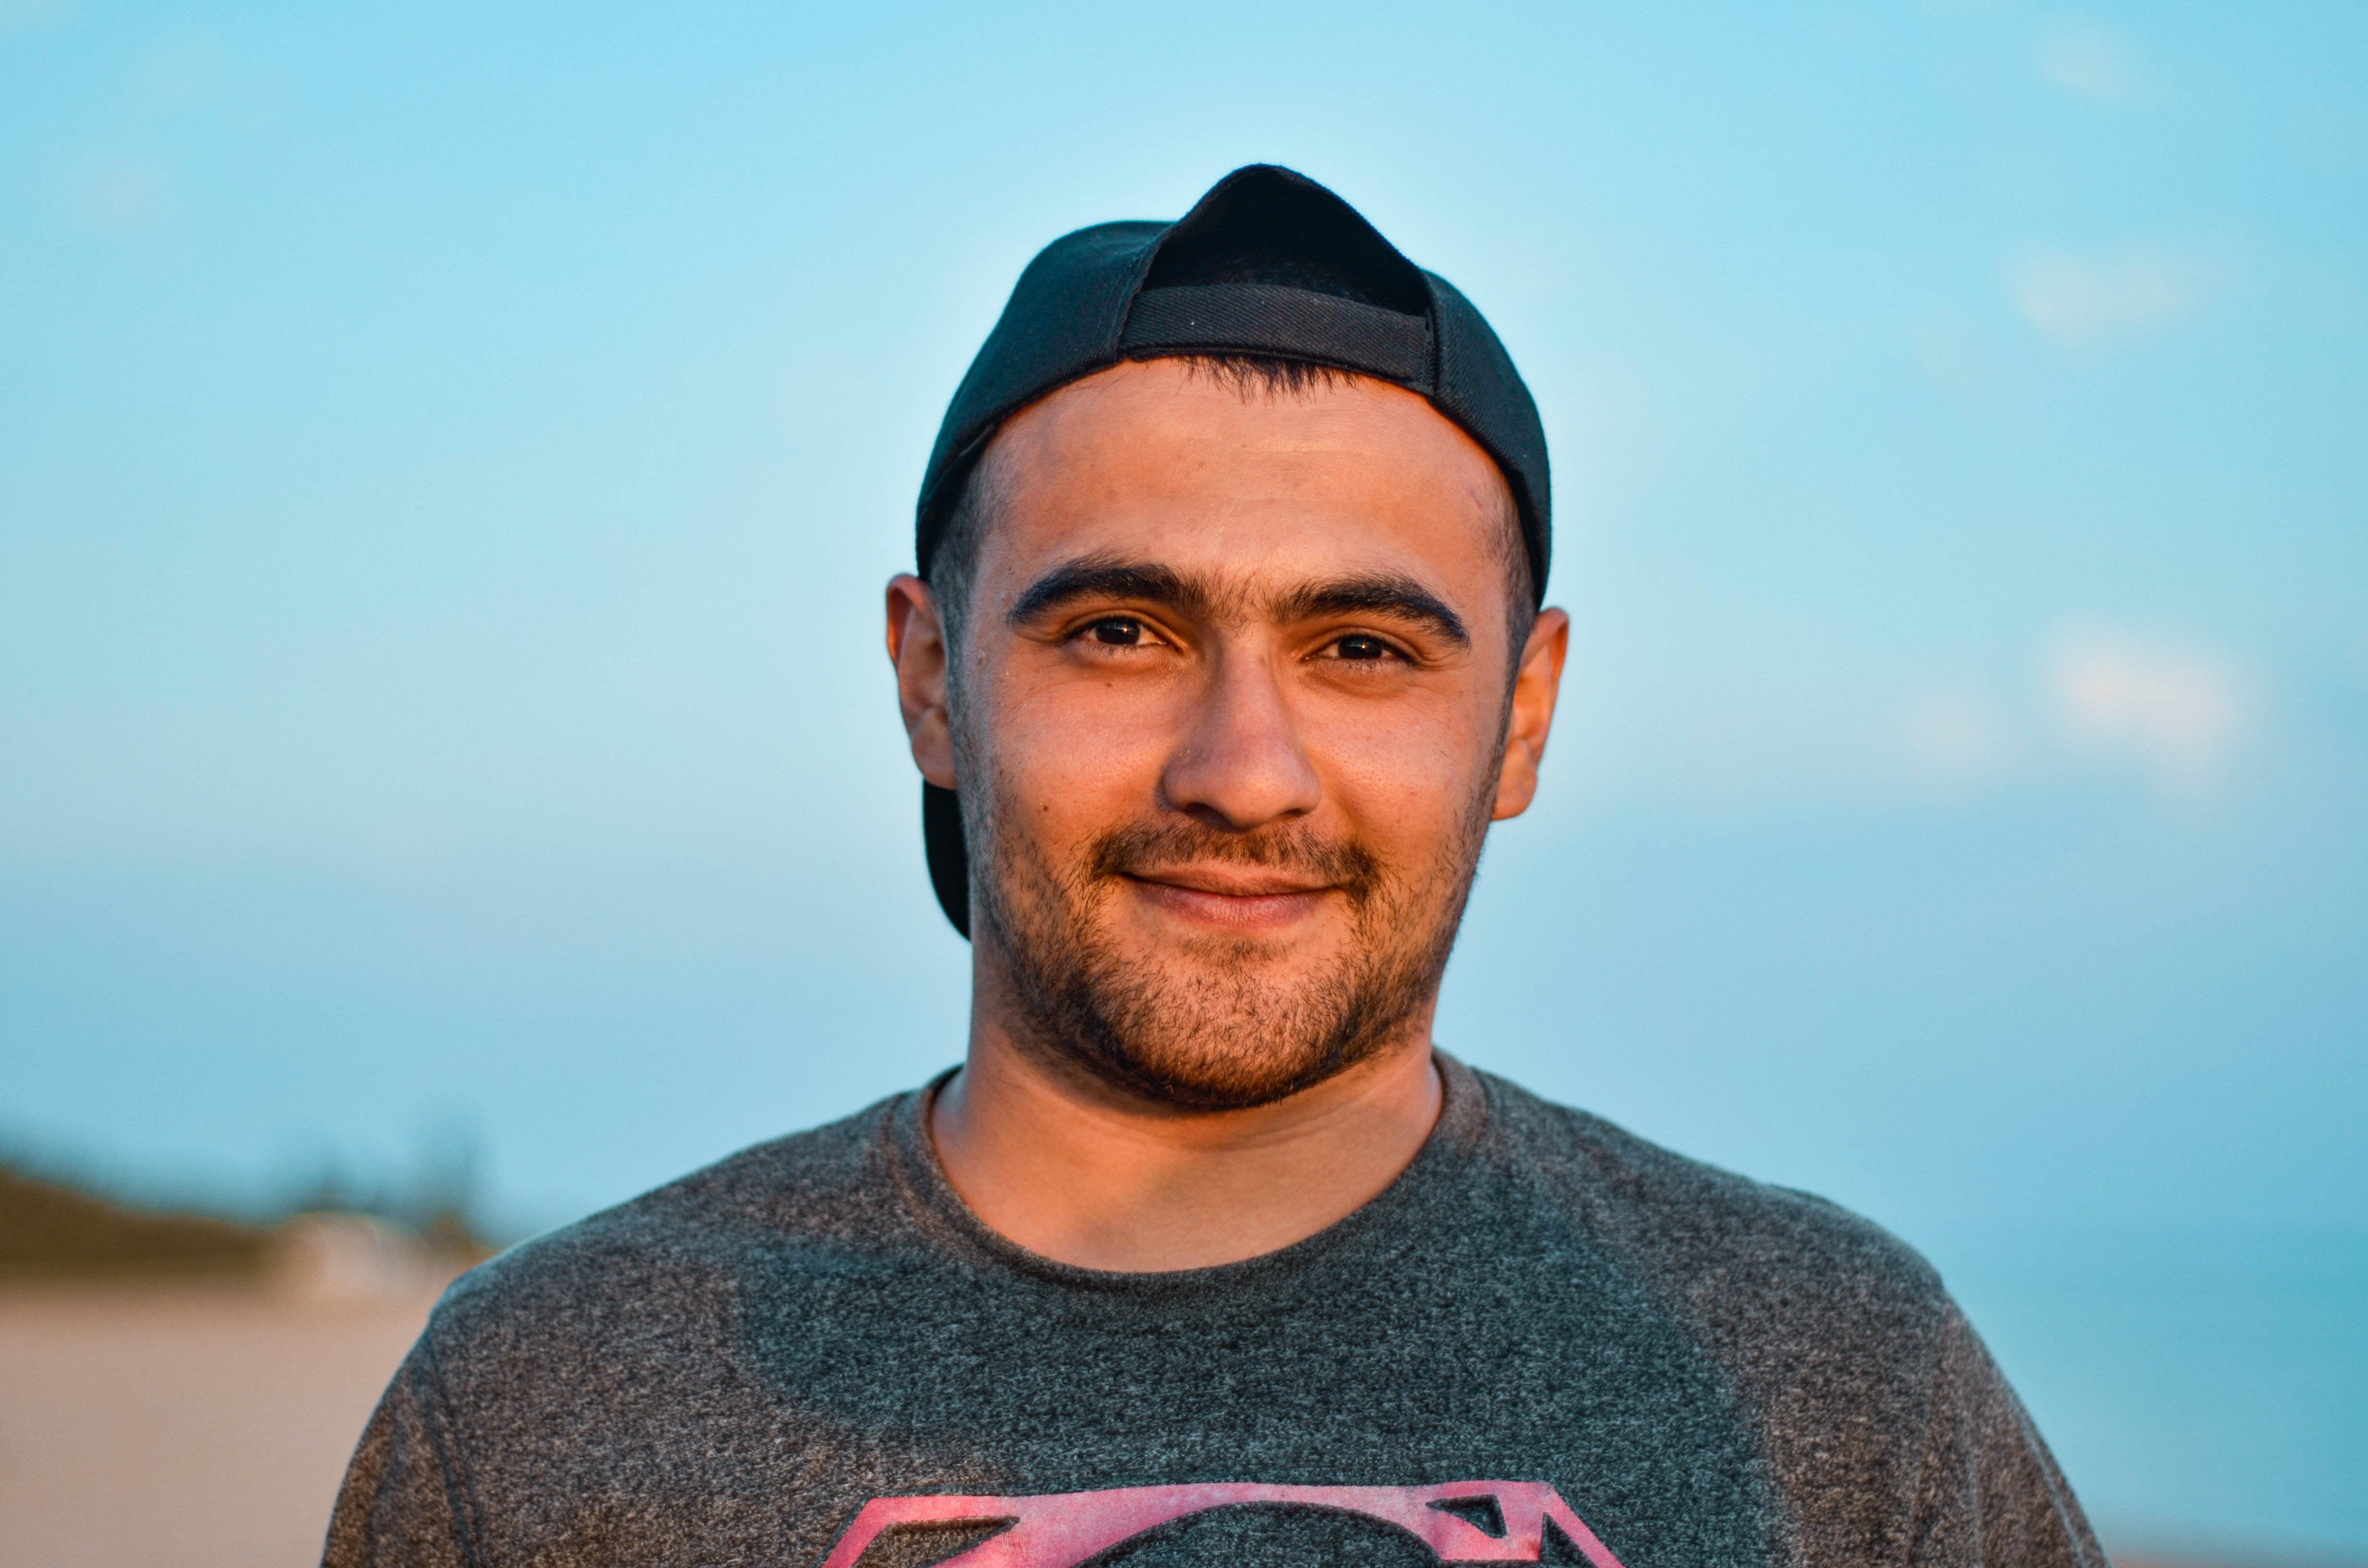
\includegraphics[height=2cm]{images/Persona_Bild.jpg}  \\
        \hline
        Demographische Angaben & 35 Jahre, männlich, Stuttgart \\
        \hline
        Beruf & Techniker \\
        \hline
        Aufgaben & - 3rd Level Support \newline - Koordination \newline - Ausbildung der Azubis und dualen Studenten \\
        \hline
        Kenntnisse & - IT-Affin \newline - Grundlegende Programmierkenntnisse \newline - Experte in Windows \\
        \hline
        Fähigkeiten & - Probleme strukturiert lösen \newline - Findet für jedes Problem eine Lösung \\
        \hline
        Erfahrung mit ähnlichen Systemen & - Enttäuscht vom letzten System \newline \\
        \hline
        Motivation & - Erhält viel lob \newline - Erst zufrieden wenn er sein bestes gegeben hat \\
        \hline
        Ziele & - Alle Probleme lösen \newline - Schnellen und guten Support \\
        \hline
        Erwartungen & - zuverlässiges Ticketsystem \newline - übersichtlich \\
        \hline
        Hobbys & - Mit der Familie Zeit verbringen \newline - Fußball in einer Hobbymannschaft\\
        \hline
        Zitat & "Ich bin erst fertig wenn alles erledigt ist und der Kunde zufrieden ist" \\
        \hline
        
    \end{tabularx}
    \chapter{Persona}
\newpage


    \chapter{Nutzungskontext}
Die Software soll im täglichen Geschäfts des Unternehmens eingesetzt werden. Die Software soll die aktuellen Aufgaben der Benutzer vereinfachen und sich optimal in den Arbeitsalltag integrieren. Die Software soll das ganze Terminhandeling übernehmen von der Einpflegung der Tickets, des Buchens von Terminen, das Durchführen von Terminen, das Dokumentieren von Terminen, sowie das anschließende erstellen eines Raports. Nach Abschluss des Termins, soll der Raport direkt in die Buchhaltung eingepflegt werden können. Die Funktionen des Ticketsystems sollen optimalerweise je nach Verwendungszweck auf unterschiedlichen Plattformen verfügbar sein. Die Administrativen Tätigkeiten werden hauptsächlich an einem Desktoppc ausgeführt, wohingehen die Techniker bei Terminen Ihr iPad verwenden möchten.
    \chapter{User Stories}

\newcounter{StoryCounter}
\setcounter{StoryCounter}{1}

\newcommand{\UserStory}[2]{

    \begin{tabularx}{\textwidth}{|X|r|}        
            \hline
            #1  & UST \theStoryCounter \\
            \hline
            \multicolumn{2}{|p{0.95\textwidth}|} {#2}\\
            \hline
    \end{tabularx}
    \refstepcounter{StoryCounter}
}

% All User Stories

\UserStory{Tickets erstellen}{Als Nutzer möchte ich Tickets erstellen können, sodass ich meien Probleme erfassen kann.  }
\UserStory{Tickets bearbeiten}{Als Techniker möchte ich Tickets bearbeiten können, sodass ich meine Tätigkeit dokumentieren kann. }
\UserStory{Terminmanagement}{Als Terminmanager möchte ich Termine verwalten können, damit ich transparent im System die Termine auf die einzlenen Kollegen aufteilen kann und diese die Tickets direkt an dem Termin abarbeiten können.}
\UserStory{Hilfe Tools}{Als Techniker möchte ich Tools verwenden können, damit ich häufige Probleme direkt und einfach aus der App bearbeiten kann.}
\UserStory{Wissensdatenbank}{Als Techniker möchte ich direkten Zugriff auf eine Wissensdatenbank haben, damit ich bei auftrettenden Problemen während des Termins überprüfen kann, ob die Lösung für das Problem bereits dokumentiert wurde.}
\UserStory{Monitoring}{Als Techniker möchte ich ein Monitoring für jeden Kunden angezeigt bekommen, damit ich überwachen kann, wo Probleme bei Kunden auftretten.}
\UserStory{Rapport}{Als Techniker möchte ich ein Rapport erstellen können, damit ich nach der Bearbeitung eines Tickets direkt den Rapport erhalte und dieser direkt von dem Kunden über einen Link unterschrieben werden kann}
\UserStory{Wartungen durchführen}{Als Techniker möchte ich die Wartungen welche einmal im Quartal durchgeführt werden in dem Programm abarbeiten kann, damit diese sauber dokumentiert werden.} 
\UserStory{Anmelden}{Als Nutzer möchte ich mich im System anmelden können, damit ich Zugriff auf alle meinen aktuellen Tickets habe und deren aktuellen Stand ansehen kann. }
\UserStory{Bewertungen}{Als Manager möchte ich, dass der Kunde den Techniker bewerten kann, um die Kundenzufriedenheit zu überprüfen und gegebenenfalls weiter zu steigern. }

\UserStory{Stammdatenverwaltung}{Als Manager möchte ich die Stammdaten der einzelnen Kunden über die Desktop App verwalten können.}


In der ersten Version würde ich alle User Stories umsetzen, durch welche die grundlegenden Funktionen wie im vorhandenen Ticketsystem abgedeckt sind. Dies würde die User-Stories 1, 2, 7, 9 umfassen.
Bewusst würde ich in der ersten Version die User-Stories 3, 4, 5, 6, 8 und 10 nicht umsetzen. Da der Benutzer vom vorhandenen Ticketsystem enttäuscht ist, ist es für Ihn zuerst wichtig das er in der ersten Version alle grundlegenden Funktionen nutzen kann und diese Ihnen zufriedenstellen. Die weiteren User-Stories welche nicht in der ersten Version eingebaut wurden, können anschließend in folgenden Versionen eingebaut werden. Dies bietet den Vorteil, dass der Benutzer in der Version 1 vom Ticketsystem überzeugt werden kann und sich für die weiteren Funktionen grundlegend mit dem System auskennt. 

	
	% Anhang
	\clearpage
	\pagenumbering{roman}

	% Abbildungsverzeichnis
	\cleardoublepage
	\phantomsection \label{listoffig}
	\addcontentsline{toc}{chapter}{Abbildungsverzeichnis}
	\listoffigures

	%Tabellenverzeichnis
	%\cleardoublepage
	%\phantomsection \label{listoftab}
	%\addcontentsline{toc}{chapter}{Tabellenverzeichnis}
	%\listoftables

	% Quellcodeverzeichnis
	%\cleardoublepage
	%\phantomsection \label{listoflist}
	%\addcontentsline{toc}{chapter}{Listings}
	%\lstlistoflistings

	% Literaturverzeichnis
	%\cleardoublepage
	%\phantomsection \label{listoflit}
	%\addcontentsline{toc}{chapter}{Literaturverzeichnis}
	
	%Bib style
	%\bibliographystyle{agsm} %Havard
	%\bibliographystyle{amsplain} %Durchnummeriert
	%\bibliographystyle{amsalpha} %Kürzel für Autor und Jahr
	%see more: http://amath.colorado.edu/documentation/LaTeX/reference/faq/bibstyles.pdf
	
	%\bibliography{ArbeitBib}

	% Abkürzungsverzeichnis
	%\cleardoublepage
	%\phantomsection \label{listofacs}
	%\addcontentsline{toc}{chapter}{Abkürzungsverzeichnis}
	%%!TEX root = ../dokumentation.tex

\chapter*{Abkürzungsverzeichnis}
%nur verwendete Akronyme werden letztlich im Dokument angezeigt
\begin{acronym}[YTMMM]
\setlength{\itemsep}{-\parsep}

\acro{AGPL}{Affero GNU General Public License}
\acro{API}{Application Programming Interface}
\acro{WYSIWYG}{What You See Is What You Get}
\end{acronym}

	
	% Glossar
	%\printglossary[style=altlist,title=Glossar]
\end{document}
